\begin{filecontents}{leer.eps}
%!PS-Adobe-2.0 EPSF-2.0
%%CreationDate: Mon Jul 13 16:51:17 1992
%%DocumentFonts: (atend)
%%Pages: 0 1
%%BoundingBox: 72 31 601 342
%%EndComments

gsave
72 31 moveto
72 342 lineto
601 342 lineto
601 31 lineto
72 31 lineto
showpage
grestore
%%Trailer
%%DocumentFonts: Helvetica
\end{filecontents}
%
\documentclass[epj]{svjour}
% Remove option referee for final version
%
% Remove any % below to load the required packages
%\usepackage{latexsym}
%\usepackage{graphics}
\usepackage{graphicx}
% etc
%
\begin{document}
%
\title{Metabolic subsystems and network science}
%\subtitle{Do you have a subtitle?\\ If so, write it here}
\author{Rok Novosel\inst{1} \and Matija \v{C}ufar\inst{2}
% \thanks is optional - remove next line if not needed
%\thanks{\emph{Present address:} Insert the address here if needed}%
}                     % Do not remove
%
\institute{Fakulteta za ra\v{c}unalni\v{s}tvo in informatiko}
%
%\date{Received: date / Revised version: date}
%
\abstract{
  Subsystems are parts of a metabolism that perform different important
  tasks in a cell. In this article, we will explore these subsystems from a
  network science point of view. We will attempt to find ways of detecting
  subsystems in a metabolic network and compare their structure. We will present
  our results on the Chinese hamster ovary cell, a mammalian cell that is
  commonly used in biomedical research and in biotechnology.
}

% tole gre v abstract
%\PACS{
%      {PACS-key}{discribing text of that key}   \and
%      {PACS-key}{discribing text of that key}
%     } % end of PACS codes

\maketitle

\section{Introduction}
\label{sec:intro}
Metabolic networks~\cite{jeong2000large} are used to model metabolism in various organisms. We usually have two types of vertices in a metabolic network: reactions and chemicals produced and consumed by the reactions. The most correct way to represent this kind of structure is with a bipartite network, where edges connect chemicals to reactions. Furthermore, the edges are directed indicating whether the chemical was produced or consumed. 

\section{Methods}

Some initial ideas for methods we could use:

\begin{itemize}
\item
  Community detection: how do different algorithms detect subsystems?
\item
  Motifs: what motifs are the most common and which motifs appear in different
  subsystems? We will look for feedback and feed-forward loops.
\item
  Maybe some other techniques to compare the subsystems with?
\end{itemize}

\section{Resutls}
\label{sec:results}

\subsection{Network global structure overview}

In this article, we will analyse a metabolic network of the Chinese hamster
ovary (CHO) cell. The CHO cell is frequently used in biological and medical
research and in the production of biopharmaceuticals\cite{chocons}.

We have used a whole-cell metabolic network of the Chinese hamster ovary (CHO)
cell that was taken from the BiGG database\cite{bigg,chocons}. The original
network contains 4,456 metabolites that take part in 6,663 reactions. The
reactions and metabolites are annotated with additional metadata, such as name,
BiGG ID, subsystem etc.

We have simplified the network to a simple directed graph, where reactions are
represented with nodes. If one reaction produces a metabolite that is used by
another reaction, they are connected by an arc. This network has 6,663 nodes and
656,609 arcs.
%TODO: dodat 546208 undirected edges?

The network has a very large connected component of 6,036 nodes, while the other
components are very small, as they are composed of at most 4 nodes. The largest
connected component contains a strongly connected component of 5,307 nodes,
while the other nodes are isolated. These probably represent sources and sinks
of the metabolism.

The network has scale-free structure. Its in-degree, out-degree and degree
distributions are plotted in figure~\ref{fig:dist}. The estimated scale factors
for the network are $\gamma_{in} = 2.5$, $\gamma_{out} = 2.3$ and $\gamma =
2.0$. % TODO: kok naj bo delta, tukej je bla 200, kar odreže večino stran.
% effective diameter = 15, clustering coefficient = 0.012, undirected 0.069

\begin{figure}
  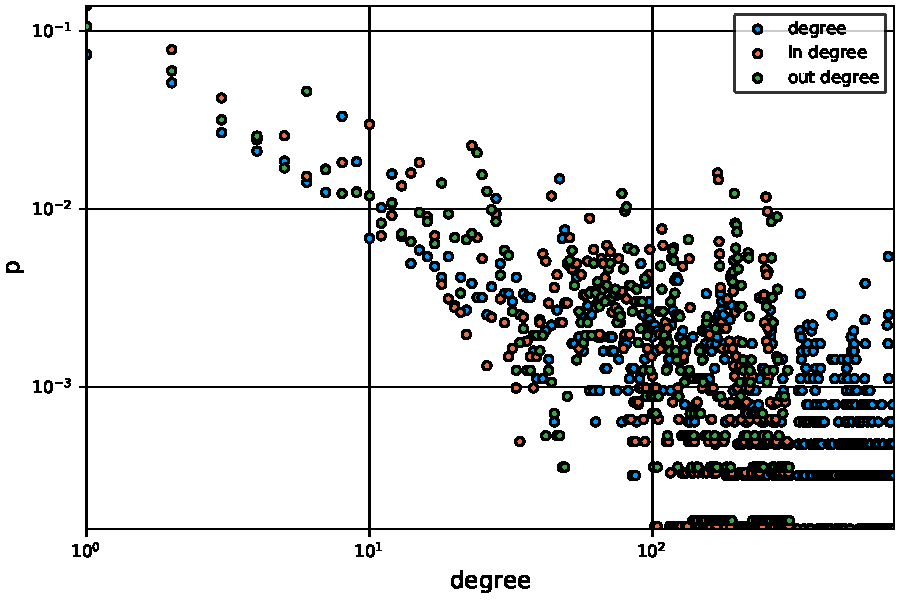
\includegraphics[width=0.45\textwidth]{../plots/degree}
  \caption{The in-degree, out-degree and degree distributions of the network.}
  \label{fig:dist}
\end{figure}


\section{Authors contributions}
All the authors were involved in the preparation of the manuscript.
All the authors have read and approved the final manuscript.

\bibliographystyle{plain}
\bibliography{biblio}

\end{document}

% TEMPLATES FOR TABLES AND FIGURES

%\begin{table}
%\caption{Please write your table caption here}
%\label{tab:1}       % Give a unique label
%\begin{tabular}{lll}
%\hline\noalign{\smallskip}
%first & second & third  \\
%\noalign{\smallskip}\hline\noalign{\smallskip}
%number & number & number \\
%number & number & number \\
%\noalign{\smallskip}\hline
%\end{tabular}
%% Or use
%\vspace*{5cm}  % with the correct table height
%\end{table}

%% For one-column wide figures use
%\begin{figure}
%% Use the relevant command for your figure-insertion program
%% to insert the figure file.
%% For example, with the option graphics use
%\resizebox{0.75\textwidth}{!}{%
%  
\includegraphics{leer.eps}
%}
%% If not, use
%%\vspace{5cm}       % Give the correct figure height in cm
%\caption{Please write your figure caption here}
%\label{fig:1}       % Give a unique label
%\end{figure}

%% For two-column wide figures use
%\begin{figure*}
%% Use the relevant command for your figure-insertion program
%% to insert the figure file. See example above.
%% If not, use
%\vspace*{5cm}       % Give the correct figure height in cm
%\caption{Please write your figure caption here}
%\label{fig:2}       % Give a unique label
%\end{figure*}
